\section{Introduction}

Likewise, the purpose of this chapter is to go through the important theories in developing the prototype together with training and testing the machine learning model.

\section{Relevant Theories and Models}

\begin{figure}[!htbp]
	\centering
	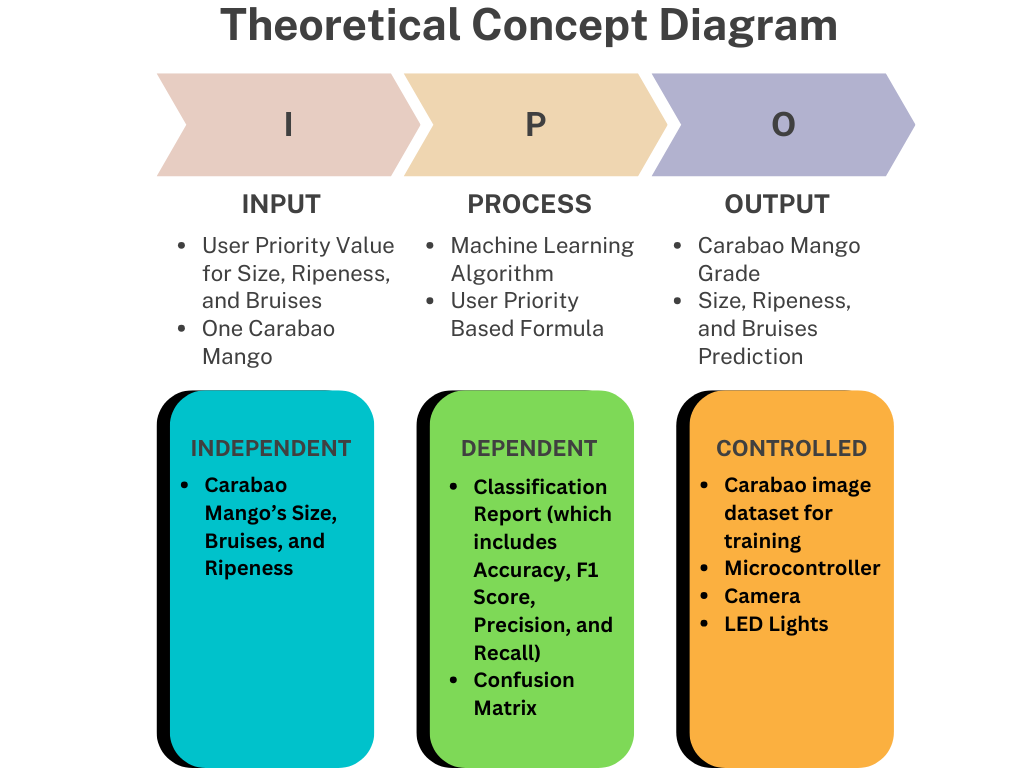
\includegraphics[width=0.5\textwidth]{theoretical_diagram3}
	\caption{Theoretical Framework Diagram.}
	\label{fig:theoreticalDiagram1}
\end{figure}

The theoretical framework seen in figure \ref{fig:theoreticalDiagram1} 
follows the IPO (Input-Process-Output) Model for a Carabao Mango Sorting
System. The Input section includes user-defined priority values for size,
ripeness, and bruises, along with a single mango for analysis. The Process
section highlights the use of a machine learning algorithm and a
user-priority-based formula to classify the mango. The Output consists of the
mango’s grade, predicted size, ripeness, and bruises. Below the IPO model, the
diagram categorizes variables into three groups: Independent (mango’s size,
ripeness, and bruises), Dependent (classification report with accuracy,
precision, recall, and confusion matrix), and Controlled (image dataset,
microcontroller, camera, and LED lights).

\section{Technical Background}

At its core, the system will be using machine learning concepts pertaining to
\gls{CNN} and OpenCV, and may use other algorithms such as Naive Bayes and
k-Nearest Neighbors to supplement the classification tasks, particularly for
assessing mango ripeness, bruise detection, and size determination. The system
will be built on an embedded framework, integrating a Raspberry Pi
microcontroller to control the RaspberryPi camera, actuators, LED lights, and
motors. A user-friendly GUI will also be utilized to ensure users can customize
the prioritization of the mango sorting system.

\section{Conceptual Framework Background}

\begin{figure}[!htbp]
	\centering
	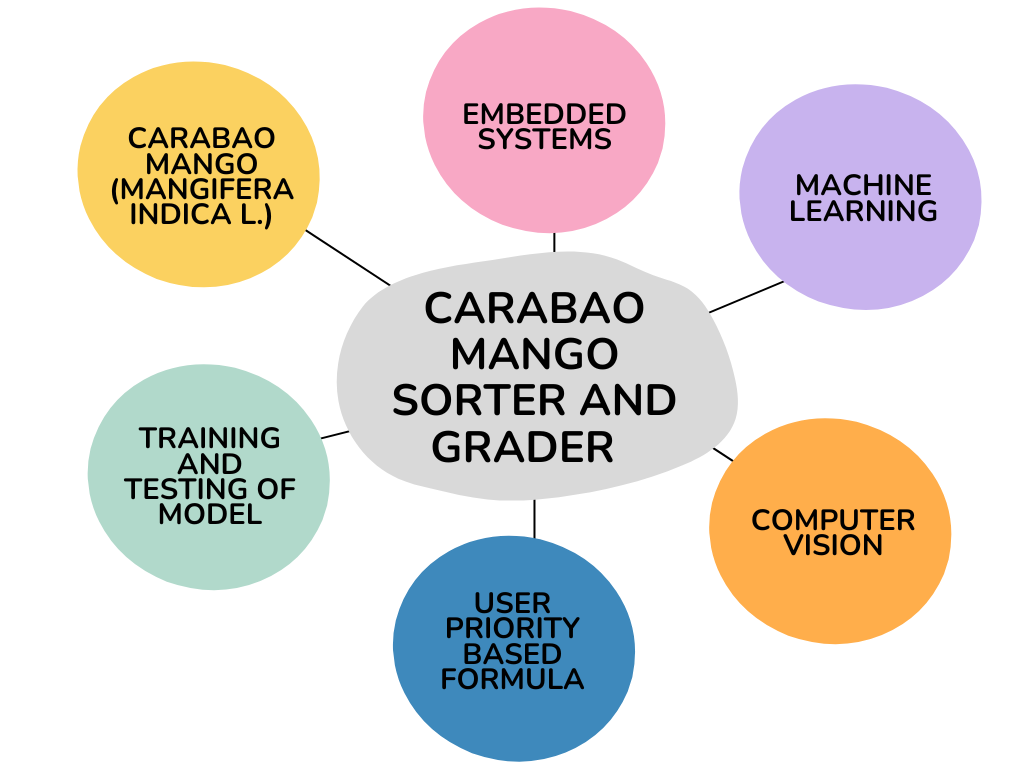
\includegraphics[width=0.5\textwidth]{concept_diagram}
	\caption{Conceptual Framework Diagram.}
	\label{fig:theoreticalDiagram2}
\end{figure}
 
The conceptual framework seen in figure \ref{fig:theoreticalDiagram2}
illustrates the key components involved in the Carabao Mango Sorter and Grader
system. At the center, the system is represented as the core element, surrounded
by six interconnected components: Carabao Mango (Mangifera indica L.), Embedded
Systems, Machine Learning, Computer Vision, User Priority-Based Formula, and
Training and Testing of the Model. These elements represent the different
technologies, methodologies, and considerations required for the development and
operation of the sorter and grader. The diagram provides an overview of how
various disciplines contribute to the project’s functionality.

\section{Software Concepts}

\subsection{Thresholding}
% add thresholding concept and how it is used in the system
Thresholding is a computer vision image segmentation technique that is used to
separate objects from their surroundings by converting a grayscale image to
binary. The conversion is done by choosing a certain threshold intensity value.
It is usually done by assigning pixels with an intensity higher than the
threshold are mapped to one value (commonly white), and pixels with an intensity
lower than the threshold are mapped to another (commonly black). The result of
this technique is in a high-contrast image that makes it easy to detect the
object's boundary and shape in the image.\\

In this project, two types of thresholding were applied:
\begin{itemize}

    \item Absolute Difference Thresholding – This method involves computing the absolute difference between two images. The first image is one of the object, and the other of the same background without the object. The result isolates only the pixels that have changed between the two images, thus isolating the mango from its background successfully.
    \item Binary Thresholding – Once the difference image has been created, binary thresholding is used. A threshold value is employed to threshold the difference image into a binary image. Values greater than the threshold are made white (foreground), and values less than that are made black (background). This creates a clear silhouette of the mango, which is appropriate for size estimation and contour detection.

\end{itemize}

\subsection{Object Size Calculation}

Object size calculation is the calculation of a certain object's true size from
image data. This is essential in computer vision systems to efficiently process
object features in real-time. In this research, the size of the Carabao mango is
estimated through image measurement techniques based on geometric principles and
camera calibration.

% (pixel_dimension * distance_camera_to_object) / focal_length_pixels = real_world_dimension
The size of the mango can be determined given:

\begin{equation}
	\label{eq:objectSizeCalculation}
	\text{Real World Dimension} = \frac{\text{Pixel Dimension} \times \text{Distance from Camera to Object}}{\text{Focal Length}}
\end{equation}

\begin{equation} \label{eq:objectSizeCalculation2}
	\ensuremath{D \left( p, d, f \right)= \frac{p \cdot d}{f} }
\end{equation}

where \gls{not:real_world_dimension} is the real world dimension of the object,
 \gls{not:pixel_dimension} is the pixel dimension of the object, 
 \gls{not:distance_from_cam_to_object} is the distance from the camera to the object,
  and \gls{not:focal_length} is the focal length of the camera.

After capture and preprocessing of the image, the binary image so obtained is
processed with contour detection to find the largest object, which is assumed to
be the mango. The contour is then bounded with a minimum-area bounding box, and
pixel-based length and width are calculated using Euclidean distance between the
corner points.

This size estimation method offers a consistent and efficient way of taking the
measurements with only standard camera input, providing consistency in
classification and reducing the necessity for physical measuring devices.


\subsection{Convolutional Neural Network}
% describe CNN and show the architecture of the CNN model
Convolutional Neural Networks are a class of deep learning models is commonly
used in analyzing visual data. CNNs are particularly effective in image
classification tasks due to their ability to automatically extract and
effectively learn the spatial hierarchies of features directly from the pixels
of a given image. This makes it highly suitable for functions such as object
detection and, in the case of this study, image classification.

CNN usually applies filters to input images.  These filters are designed to
detect local patterns such as edges, textures, and color gradients. The network
is able to learn more patterns as the data goes through the layers. This enables
it to recognize effectively the characteristics that it is looking for.

The use of CNNs in this study allows for accurate, automated classification of
mango images which contributes to the development of a reliable, non-destructive
grading system that minimizes human error and ensures consistent quality
assessment


\subsection{Classification Report}
% describe classification report and how it is used in the system

\subsubsection{Confusion Matrix}

\begin{table}[h]
	\centering
	\begin{tabular}{c|c|c}
	\hline
	& \textbf{Predicted Positive} & \textbf{Predicted Negative} \\
	\hline
	\textbf{Actual Positive} & TP & FN \\
	\hline
	\textbf{Actual Negative} & FP & TN \\
	\hline
	\end{tabular}
	\caption{Confusion Matrix Example}
	\label{tab:confusion_matrix}
\end{table}

A confusion matrix is a table that visualizes the performance 
of a classification model. For a binary classification problem, it has four
components: \\

\begin{itemize}
	\item True Positives (TP): Cases correctly predicted as positive
	\item True Negatives (TN): Cases correctly predicted as negative
	\item False Positives (FP): Cases incorrectly predicted as positive. (Type I error)
	\item False Negatives (FN): Cases incorrectly predicted as negative (Type II error)
\end{itemize}


\subsubsection{Precision}
\begin{eqnarray}
	\text{Precision} = \frac{TP}{TP + FP}
	\label{eq:precision}
\end{eqnarray}

Precision measures how many of the predicted positives are actually positive. It answers the question: 
"When the model predicts the positive class, how often is it correct?" High precision means low false positives.

\subsubsection{Recall}
\begin{eqnarray}
	\text{Recall} = \frac{TP}{TP + FN}
	\label{eq:recall}
\end{eqnarray}

Recall, which is also called sensitivity, measures how many of the actual positives were correctly identified. 
It answers the question: 
"Of all the actual positive cases, how many did the model catch?" High recall means low false negatives.

\subsubsection{F1 Score}
\begin{eqnarray}
	F_1 = 2\times \frac{\text{Precision} \times \text{Recall}}{\text{Precision} + \text{Recall}}
	\label{eq:f1_score}
\end{eqnarray}

The F1 score is the harmonic mean of precision and recall. It provides a single metric that balances 
both concerns. This is particularly useful when you need to 
find a balance between precision and recall, as optimizing for one often decreases the other.

\subsubsection{Accuracy}
\begin{eqnarray}
	\text{Accuracy} = \frac{TP + TN}{TP + TN + FP + FN}
	\label{eq:accuracy}
\end{eqnarray}

Accuracy measures the proportion of correct predictions (both true positives and true negatives)
 among the total cases. While intuitive, accuracy can be misleading with imbalanced datasets.

\section{Hardware Concepts}

\subsection{Camera Module} 

The camera module serves as the main image acquisition tool in the mango sorter
and grader system. Its role is to capture clear, high-resolution images of each
mango as it moves along the conveyor. These images are critical for analyzing
physical traits like ripeness, bruising, and size through computer vision and
machine learning techniques.

The camera is directly connected to the Raspberry Pi, which manages both image
capture and processing. It is fixed in position to ensure consistent distance
and angle for all images. It is also paired with a lighting system to provide a
consistent lighting for the images. The system captures images of both the top
and bottom sides of each mango to ensure a more accurate grading. The prototype
integrates the Raspberry Pi Camera Module Version 2. This camera is chosen for
its 8MP resolution which is critical in capturing real-time images. Another
reason for integrating this camera is because of its compatibility with the
Raspberry Pi 4, and reliability in capturing detailed images needed for accurate
classification. It is also cost effective and lightweight which is important for
the prototype.

\subsection{4 Channel Relay}
% add Relay H-bridge circuit diagram
The relay module in this project is used to control the direction and movement
of the motors that operate the conveyor system and mango sorting mechanism. As
an electrically operated switch, the relay allows the low-power signals from the
Raspberry Pi to safely manage the higher voltage and current required by the DC
motors.

For the prototype, the relay module is responsible for changing the polarity of
motor connections which enables the motors to rotate in both forward and reverse
directions. This will drive the conveyor belt system. This is essential for
moving mangoes along the conveyor, rotating them for the top and bottom image
capture, and directing them to the appropriate bin based on their grade.

\subsection{Gear Ratio}
% add picture of a pulley belt and concept behind it (what is a pulley belt)

In this prototype, gear ratios are used to control the rotational speed of the
conveyor belts that move and rotate the mango. A gear ratio of 1:3 was applied,
meaning the motor gear completes one full rotation for every three rotations of
the driven gear. This is also done in order to avoid overspeeding and make sure
that the conveyor belt moves in a controlled manner. This setup slows down one
belt relative to the other, creating a differential speed between the left and
right belts. As a result, the mango rotates in place while being moved forward.
This rotation is essential for capturing both the top and bottom views of the
mango for accurate classification and grading.

% PUT THE FOLLOWING IN THE THEORETICAL CONSIDERATION
% H bridge type connection with the two DC motors
% 1:3 belt connection unless changed
% Stepper Motor Specifications
% https://www.makerlab-electronics.com/products/stepper-motor-nema-17-2600g-cm
% https://lastminuteengineers.com/drv8825-stepper-motor-driver-arduino-tutorial/

\section{Summary}

Overall, chapter 3 establishes key concepts and theoretical considerations that form the foundation of the Carabao mango sorter and grading system. It discusses and connects each component together, explaining how each component such as the RaspberryPi and DC motors work together to create a system that utilizes machine learning and computer vision techniques to classify mangoes based on user priority.
